\documentclass[11pt]{article}

\usepackage[margin=1in]{geometry}
\usepackage{graphicx}
\usepackage{booktabs}
\usepackage{longtable}
\usepackage{array}
\usepackage{xcolor}
\usepackage{hyperref}
\usepackage{url}

\hypersetup{
  colorlinks=true,
  linkcolor=blue,
  urlcolor=blue,
  citecolor=blue
}

\setlength{\parskip}{0.55em}
\setlength{\parindent}{0pt}
\renewcommand{\arraystretch}{1.15}

\newcommand{\projectname}{Visual-Fusion-GRU}
\newcommand{\studentname}{Quanlong Zhao}
\newcommand{\studentid}{999014947}
\newcommand{\successbest}{95.7\%}

\title{\textbf{\projectname: Final Project Report}\\
\large SLA-Aware Underwater VLA Navigation with RL, CLIP Heatmaps, GRU Imitation, and Hard-Case DAgger}
\author{\studentname\\Student ID: \studentid}
\date{June 2026}

\begin{document}

\begin{titlepage}
\centering
\vspace*{0.75in}
{\Huge \textbf{\projectname}\par}
\vspace{0.2in}
{\Large Final Project Report\par}
\vspace{0.15in}
{\large SLA-Aware Underwater VLA Navigation with RL, CLIP Heatmaps, GRU Imitation, and Hard-Case DAgger\par}
\vspace{0.6in}
{\Large \studentname\par}
{\large Student ID: \studentid\par}
\vspace{0.4in}
{\large Department Project Submission\par}
{\large June 2026\par}
\vfill
\begin{minipage}{0.9\textwidth}
\centering
\textbf{Headline result:} the current best GRU imitation student reaches
\textbf{0.957 success rate over 1000 pure-CLIP evaluation episodes} after
hard-case DAgger fine-tuning.
\end{minipage}
\vfill
\end{titlepage}

\tableofcontents
\newpage

\section{Abstract}

This report describes the design, training history, and final experimental
outcome of \projectname, a GitHub-ready underwater navigation project for an
autonomous robotic fish in NVIDIA Isaac Sim. The project goal is a
Vision-Language-Action (VLA) style policy: given an instruction such as
\texttt{Find the red ball}, the robot should ground the instruction in camera
observations and choose low-level swimming actions. The work began with
reinforcement learning (RL) and an alpha-fusion curriculum that attempted to
migrate from a stable color-saliency fallback heatmap to a CLIP semantic
heatmap. The RL experiment revealed a repeatable bottleneck near
\texttt{alpha = 0.993}, where only \texttt{0.007} fallback weight remained, but
success dropped sharply. This showed that even a very small fallback component
still carried high-quality control decisions.

The final successful path used imitation learning instead of direct RL
annealing. A fallback RL policy was preserved as the teacher. A CLIP-observation
student was trained with behavior cloning (BC), then DAgger, then a recurrent
GRU policy, and finally hard-case DAgger fine-tuning. The current best released
checkpoint is \path{models/student_gru_hard_cases_radius1_seed601000.pt}. It
achieves \textbf{0.957 success rate over 1000 pure-CLIP episodes}, with mean
steps \textbf{31.341}. The final fine-tuning stage used \textbf{73737} labeled
records from the balanced teacher seed dataset, eight balanced GRU DAgger
shards, and a radius-1 hard-case dataset.

\section{Repository and Project Scope}

The GitHub package is stored in:

\begin{center}
\path{/home/quanlong/isaac-sim/Visual_Fusion_GRU_github}
\end{center}

The repository is curated from a larger Isaac Sim workspace. It contains source
code, model checkpoints, configs, evaluation summaries, monitor logs, DAgger
datasets, and upload notes. The full Isaac Sim installation and local
TensorBoard event folders are not intended to be the core public artifact.

\begin{figure}[htbp]
\centering
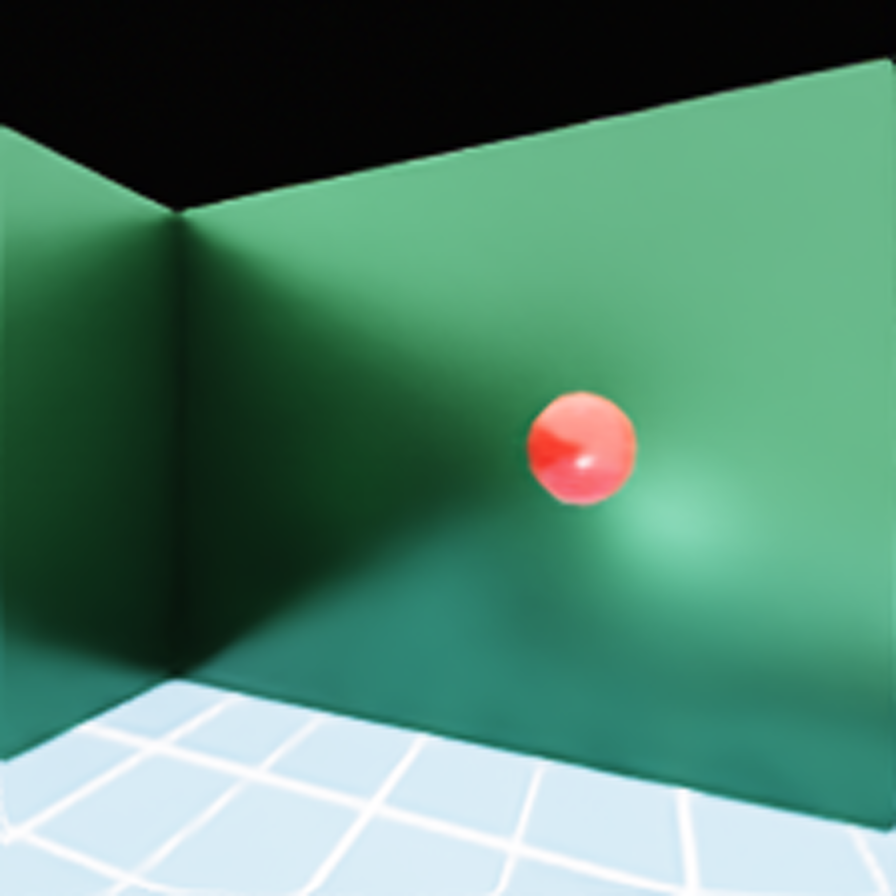
\includegraphics[width=0.88\linewidth]{figures/current_student_simulation.png}
\caption{Current GRU student simulation screenshot included with the GitHub package.}
\label{fig:sim}
\end{figure}

\subsection{Main Repository Components}

\begin{longtable}{p{0.28\linewidth}p{0.64\linewidth}}
\toprule
\textbf{Path} & \textbf{Purpose} \\
\midrule
\endhead
\path{src/underwater_env.py} & Isaac Sim underwater navigation environment, including observation construction and low-level action stepping. \\
\path{src/vla_clip.py} & CLIP-based semantic heatmap construction for the language-conditioned observation path. \\
\path{src/train_phaseb_hybrid.py} & Historical hybrid RL training entry point for the alpha-fusion curriculum. \\
\path{src/train_fallback_teacher.py} & Fallback teacher RL training entry point. \\
\path{src/imitation/} & Behavior cloning, DAgger, datasets, configs, policy adapters, evaluation helpers, and model definitions. \\
\path{src/imitation/models.py} & MLP and GRU student policies for heatmap-to-action classification. \\
\path{configs/imitation/} & JSON configs for BC, DAgger, GRU DAgger, evaluation, teacher dataset collection, and fallback teacher training. \\
\path{models/} & Compact trained artifacts, including fallback teacher, historical RL checkpoints, BC baselines, and the current best GRU student. \\
\path{imitation_data/} & Teacher seed datasets and evaluation summaries. \\
\path{imitation_runs/} & DAgger datasets, checkpoints, and per-run summaries. \\
\path{monitor_logs/} & Monitor CSV logs for fallback and hybrid RL runs. \\
\path{docs/} & GitHub upload notes, project structure, next-experiment notes, and assets. \\
\bottomrule
\end{longtable}

\section{Problem Definition}

The robotic fish must navigate underwater toward a target object while using a
vision-language style observation. The target instruction used throughout the
recorded experiments is:

\begin{center}
\texttt{Find the red ball}
\end{center}

The action space is discrete:

\begin{itemize}
  \item \textbf{0}: swim forward,
  \item \textbf{1}: turn left,
  \item \textbf{2}: turn right.
\end{itemize}

The semantic observation used by the imitation student is a flattened CLIP
heatmap with input dimension \textbf{196}, corresponding to a \(14 \times 14\)
spatial heatmap. This compact representation is used by both the MLP and GRU
student models.

The environment is challenging because underwater visual navigation does not
only require moving toward a visible object. The policy must also avoid
left-right oscillation when the target leaves the camera view, recover from
target loss, and decide when to keep moving forward instead of over-correcting
with turns.

\section{Original RL Plan}

The original project hypothesis was that a stable color-saliency fallback
policy could teach the physical target-tracking behavior, and then an RL
curriculum could gradually replace fallback geometry with semantic CLIP
heatmaps. The hybrid observation was:

\[
  obs = \alpha \cdot CLIP\_heatmap + (1 - \alpha) \cdot fallback\_heatmap.
\]

The intended roadmap was:

\begin{enumerate}
  \item train a fallback RL policy on color saliency;
  \item use the fallback policy as a stable target-tracking base;
  \item introduce CLIP semantic heatmaps with alpha fusion;
  \item slowly increase \(\alpha\) until \(\alpha = 1.0\);
  \item remove the fallback path and keep a pure semantic policy.
\end{enumerate}

This was a reasonable first plan. The fallback signal was dense and physically
meaningful: when the red target was visible, its heatmap peak gave a clean
left-center-right steering cue. CLIP was more semantically aligned with
language, but less reliable as a metric control signal. The alpha curriculum
was intended to bridge that representation gap.

\section{RL Choke Point}

The Phase B hybrid RL experiment tested the migration directly. The key run is
documented by:

\begin{itemize}
  \item config: \path{models/run_config_phaseb_hybrid.json},
  \item monitor log: \path{monitor_logs/monitor_phaseb_resume_992_softgate_20260420_130251.monitor.csv},
  \item launch script: \path{scripts/run_phaseb_resume_990to1000.sh}.
\end{itemize}

The curriculum moved from \(\alpha = 0.992\) toward \(\alpha = 1.0\), using
small \texttt{0.0005} alpha milestones and a \texttt{0.9} success-rate gate.
The run stalled before reaching pure CLIP:

\begin{table}[htbp]
\centering
\caption{Hybrid RL alpha-curriculum bottleneck.}
\begin{tabular}{rrrr}
\toprule
\textbf{Alpha} & \textbf{Episodes} & \textbf{Successes} & \textbf{Success rate} \\
\midrule
0.9920 & 80 & 73 & 0.912 \\
0.9925 & 128 & 114 & 0.891 \\
0.9930 & 2368 & 1602 & 0.677 \\
0.9935 & 1244 & 643 & 0.517 \\
\bottomrule
\end{tabular}
\label{tab:alpha}
\end{table}

This was the most important negative result in the project. At
\(\alpha = 0.993\), the fallback contribution is only \(1 - \alpha = 0.007\),
or \(0.7\%\) of the fused heatmap. Yet removing this tiny part caused a major
drop in success. The interpretation is that the fallback signal was small in
percentage but large in decision quality. It still supplied critical
low-level steering information in states where the CLIP heatmap was too noisy
or too semantically broad to support stable control.

The observed failure mode was not just a bad hyperparameter setting. It was a
representation mismatch. The fallback heatmap represented target geometry in a
control-friendly way, while the CLIP heatmap represented semantic likelihood.
The policy needed a stable steering gradient, especially after target loss. As
\(\alpha\) approached 1.0, PPO kept collecting on-policy data from increasingly
unstable behavior, including search loops and left-right shaking. This made
direct RL annealing a poor route to the final pure-CLIP objective.

\section{Shift to Imitation Learning}

The project did not discard the fallback teacher. Instead, the successful
decision was to keep the useful part of the RL work and change the transfer
method. The fallback policy became a teacher, while the student observed only
the CLIP heatmap. The central question changed from:

\begin{quote}
Can PPO discover how to migrate from fallback to CLIP?
\end{quote}

to:

\begin{quote}
Can a CLIP-view student imitate the decisions of a fallback teacher, including
off-trajectory recovery states?
\end{quote}

\begin{figure}[htbp]
\centering
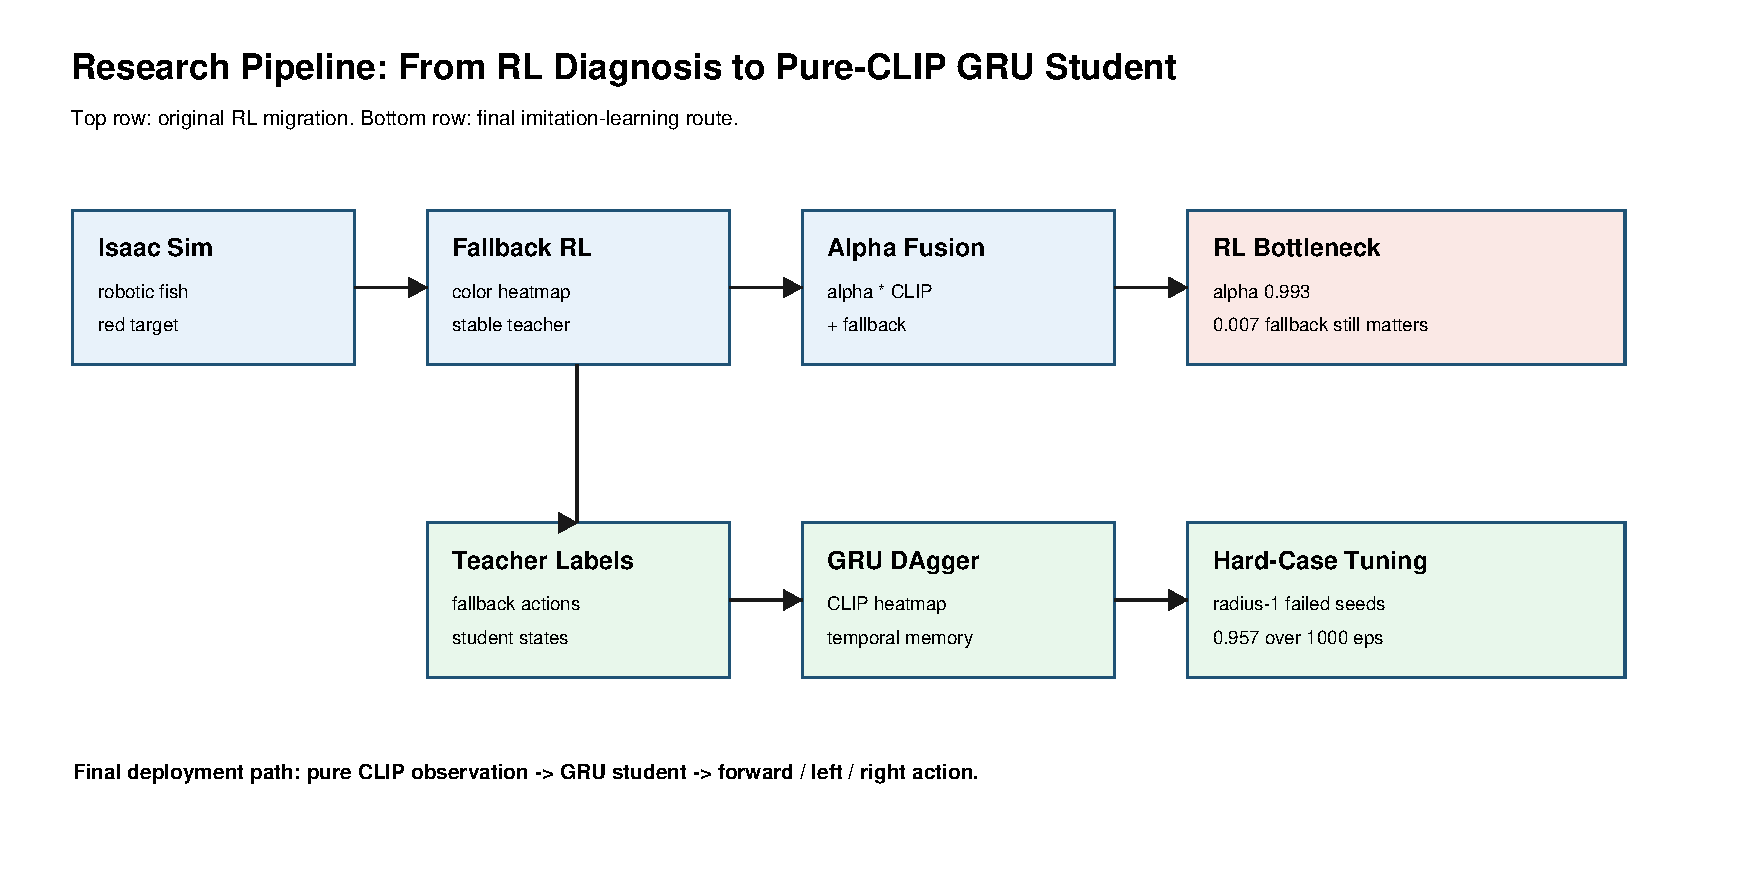
\includegraphics[width=0.92\linewidth]{figures/training_pipeline.pdf}
\caption{Training pipeline: RL exposed the semantic-control bottleneck, then imitation learning used the fallback policy as teacher and trained a pure-CLIP GRU student.}
\label{fig:pipeline}
\end{figure}

\subsection{Behavior Cloning Baseline}

The first imitation baseline used behavior cloning on teacher-labeled
examples. The balanced teacher seed dataset contains \textbf{360} teacher
episodes and \textbf{11720} labeled records:

\begin{center}
\path{imitation_data/teacher_seed_balanced/teacher_seed_balanced_dataset.summary.json}
\end{center}

The early BC-only CLIP student was weak. In the recorded balanced evaluation,
\path{models/student_bc_balanced.pt} achieved only \textbf{0.15} success rate
over \textbf{20} episodes. Its action histogram was:

\begin{center}
\texttt{\{"0": 108, "1": 4904, "2": 4912\}}
\end{center}

The almost symmetric left/right counts indicate the main problem: the model
often oscillated instead of committing to a useful tracking or search action.
This made DAgger necessary.

\subsection{DAgger}

DAgger corrects a limitation of pure BC. BC trains on teacher states, but at
test time the student visits states created by its own mistakes. DAgger
collects the states the student actually visits, asks the teacher for labels
in those states, adds the corrected examples to the dataset, and trains again.

The balanced GRU DAgger configuration is stored at:

\begin{center}
\path{configs/imitation/dagger_gru_balanced.json}
\end{center}

Key settings were:

\begin{itemize}
  \item \textbf{model type}: GRU,
  \item \textbf{total iterations}: 8,
  \item \textbf{rollout episodes per iteration}: 40,
  \item \textbf{scenario plan}: balanced,
  \item \textbf{in-view runs per iteration}: 20,
  \item \textbf{out-of-view runs per iteration}: 20,
  \item \textbf{beta schedule}: 0.8 to 0.2,
  \item \textbf{evaluation episodes per iteration}: 25.
\end{itemize}

The balanced scenario plan was important. It forced DAgger to collect both
normal visible-target tracking states and harder target-loss/search states.

\section{GRU Student Model}

The recurrent student is implemented in:

\begin{center}
\path{src/imitation/models.py}
\end{center}

The final student uses \texttt{HeatmapActionGRU}. It consumes the flattened
CLIP heatmap at each timestep and keeps a recurrent hidden state during
rollout. This gives the model short-term memory of where the target was before
it disappeared from the current camera view. The model predicts one of the
three discrete actions at each step.

The main architecture configuration is:

\begin{table}[htbp]
\centering
\caption{GRU student architecture and training configuration.}
\begin{tabular}{ll}
\toprule
\textbf{Parameter} & \textbf{Value} \\
\midrule
Input dimension & 196 \\
GRU hidden dimension & 128 \\
GRU layers & 1 \\
MLP head hidden dimensions & [128] \\
Activation & ReLU \\
Dropout & 0.0 \\
Batch size & 128 \\
Initial epochs & 20 \\
Initial learning rate & 0.001 \\
Weight decay & 0.0001 \\
Sequence length & 16 \\
Sequence stride & 4 \\
Device in config & CPU \\
\bottomrule
\end{tabular}
\label{tab:gru}
\end{table}

Compared with an MLP, the GRU directly targets the project's hardest control
case: target loss. A single heatmap can be ambiguous when the target is partly
or fully out of frame. A short history lets the student remember whether it was
last turning left, turning right, or aligned enough to move forward.

\section{Training Data}

The final best model was not produced by one large undifferentiated training
run. It was built through a sequence of increasingly targeted datasets:

\begin{table}[htbp]
\centering
\caption{Dataset ladder used for the best GRU student.}
\begin{tabular}{lrrl}
\toprule
\textbf{Dataset stage} & \textbf{Episodes} & \textbf{Records} & \textbf{Role} \\
\midrule
Balanced teacher seed & 360 & 11720 & Initial fallback teacher labels \\
Balanced GRU DAgger shards & 320 & 26444 & Off-policy student recovery data \\
First hard-case shard & 119 & 4905 & Failed-seed correction after broad GRU eval \\
Radius-1 hard-case shard & 299 & 35573 & Expanded hard cases around seed family 601000 \\
\bottomrule
\end{tabular}
\label{tab:data}
\end{table}

The final radius-1 fine-tune used \textbf{73737} total labeled records across
ten dataset paths. The training summary is:

\begin{center}
\path{imitation_runs/dagger_gru_hard_cases_radius1_seed601000/summaries/hard_seed_dataset_train_summary.json}
\end{center}

This final stage resumed from the previous hard-case student:

\begin{center}
\path{imitation_runs/dagger_gru_hard_cases_1000/checkpoints/student_hard_seed.pt}
\end{center}

It then fine-tuned for \textbf{2} additional epochs at learning rate
\textbf{5e-5}, producing:

\begin{center}
\path{imitation_runs/dagger_gru_hard_cases_radius1_seed601000/checkpoints/student_hard_seed.pt}
\end{center}

A GitHub-friendly copy of this checkpoint is stored as:

\begin{center}
\path{models/student_gru_hard_cases_radius1_seed601000.pt}
\end{center}

\section{Evaluation Results}

\begin{figure}[htbp]
\centering
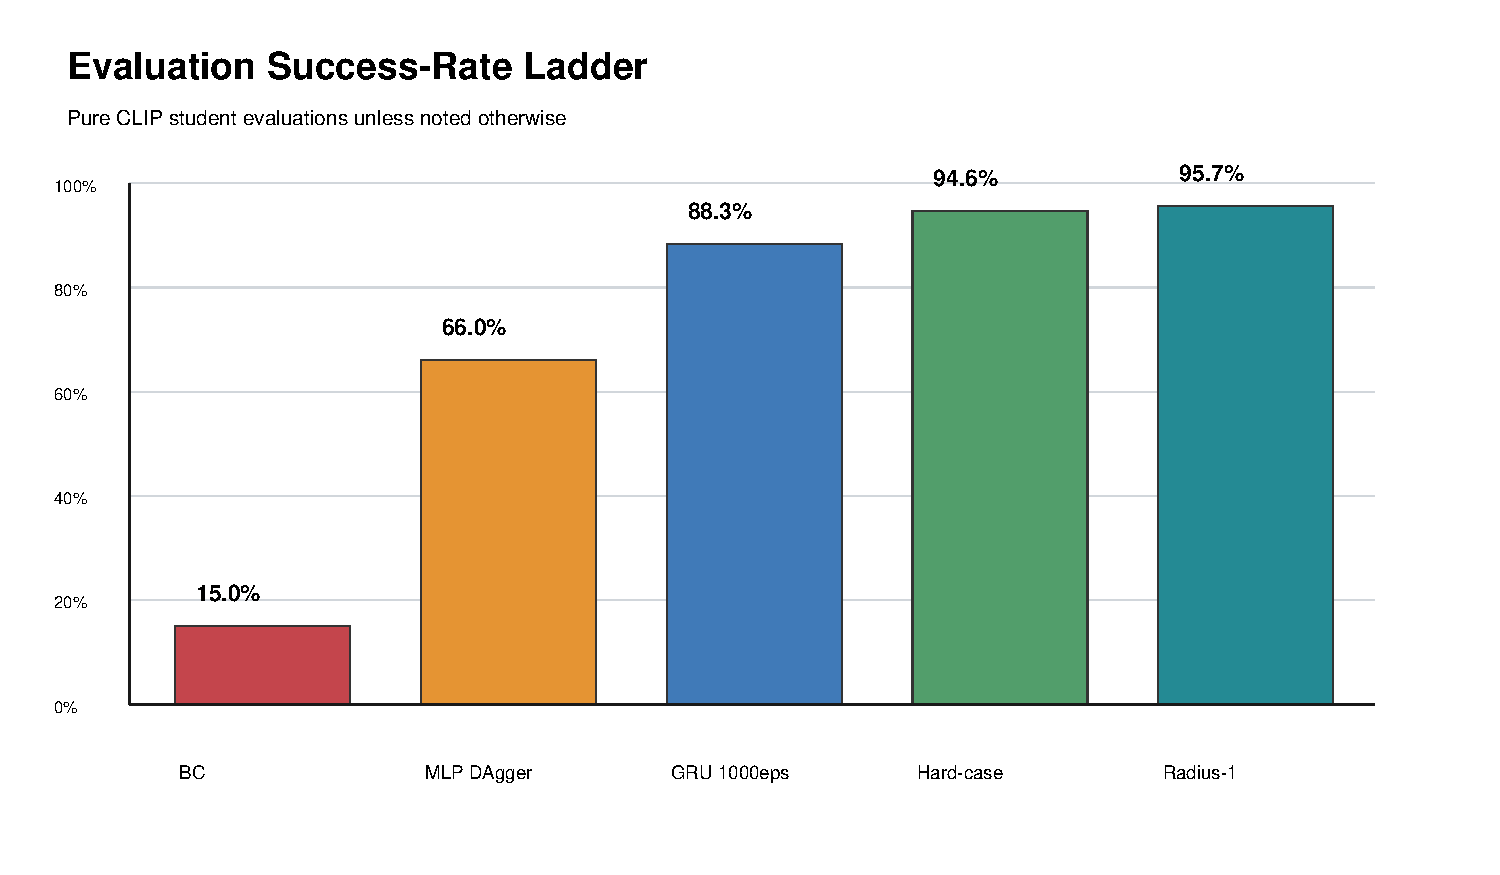
\includegraphics[width=0.95\linewidth]{figures/success_rate_ladder.pdf}
\caption{Success-rate ladder from BC through final radius-1 hard-case GRU fine-tuning.}
\label{fig:ladder}
\end{figure}

The evaluation ladder shows the effect of each major design change:

\begin{table}[htbp]
\centering
\caption{Main policy evaluation results.}
\begin{tabular}{lrrrr}
\toprule
\textbf{Policy} & \textbf{Episodes} & \textbf{Success rate} & \textbf{Mean reward} & \textbf{Mean steps} \\
\midrule
BC-only MLP baseline & 20 & 0.150 & 54.156 & 496.200 \\
MLP DAgger iter04 & 100 & 0.660 & 34.682 & 46.130 \\
GRU DAgger iter08 & 100 & 0.880 & 51.609 & 32.010 \\
GRU DAgger iter08 & 200 & 0.920 & 53.484 & 29.370 \\
GRU DAgger iter08 & 1000 & 0.883 & 51.587 & 31.346 \\
Hard-case GRU & 1000 & 0.942 & 60.931 & 79.066 \\
Hard-case GRU, seed 601000 family & 1000 & 0.946 & 60.857 & 69.151 \\
Radius-1 hard-case GRU & 1000 & \textbf{0.957} & 56.392 & 31.341 \\
\bottomrule
\end{tabular}
\label{tab:eval}
\end{table}

The final policy's action histogram over the 1000-episode evaluation was:

\begin{center}
\texttt{\{"0": 17409, "1": 2404, "2": 11528\}}
\end{center}

The best result is supported by:

\begin{itemize}
  \item \path{imitation_data/eval/dagger_gru_hard_cases_radius1_seed601000_1000eps/student_hard_seed_eval_1000eps.json},
  \item \path{imitation_data/eval/dagger_gru_hard_cases_radius1_seed601000_1000eps/student_hard_seed_hard_cases.json},
  \item \path{models/CURRENT_BEST_STUDENT.md}.
\end{itemize}

\subsection{Residual Hard Cases}

The latest hard-case report contains \textbf{48} hard cases over 1000
episodes:

\begin{itemize}
  \item 43 outright failures,
  \item 0 near misses under the configured near-miss rule,
  \item 5 slow successes.
\end{itemize}

This is a useful residual set. The broad behavior has mostly been learned, so
the next improvements should focus on targeted recovery rather than simply
adding more random episodes. However, because hard-case tuning can overfit, any
new fine-tune should also be evaluated on a wider unseen seed range.

\section{Why the Final Approach Worked}

The final result came from combining three insights:

\subsection{RL Found the Bottleneck}

The alpha-fusion RL experiment did not reach \(\alpha = 1.0\), but it produced
a valuable diagnosis. The failure near \(\alpha = 0.993\) showed that the last
small fallback component was not redundant. It was doing important work in the
control loop. This prevented the project from spending more time trying to
force PPO through an unstable representation transition.

\subsection{DAgger Matched the Student's Actual State Distribution}

BC trained on teacher states, but the student made mistakes and entered states
not well represented in the initial teacher dataset. DAgger fixed this by
collecting labels for states the student actually visited. The MLP DAgger
baseline already improved strongly over BC, and the GRU version improved the
target-loss behavior further.

\subsection{GRU Memory Reduced Target-Loss Oscillation}

The target can temporarily leave the camera field of view. A single CLIP
heatmap at that moment can be weak or ambiguous. The GRU hidden state gives the
student temporal context: it can remember recent target direction and avoid
resetting to symmetric left-right shaking. This directly addresses the failure
mode observed in early BC and RL rollouts.

\subsection{Hard-Case Mining Focused the Remaining Learning}

After the broad GRU policy reached 0.883 success over 1000 episodes, its failed
seeds were extracted and used as targeted teacher-labeled data. The first
hard-case fine-tune raised performance into the 0.94 range. Expanding the
hard-case seed set with radius 1 produced 299 targeted episodes and pushed the
current best to 0.957.

\section{Reproducibility}

The release package contains helper scripts for the current workflow:

\begin{longtable}{p{0.44\linewidth}p{0.48\linewidth}}
\toprule
\textbf{Command} & \textbf{Purpose} \\
\midrule
\endhead
\path{./scripts/eval_student_release.sh} & Evaluate the public current-best checkpoint using \path{configs/imitation/eval_current_best_student.json}. \\
\path{./scripts/run_dagger_gru_release.sh} & Run the balanced GRU DAgger release configuration. \\
\path{./scripts/eval_dagger_gru_students_200eps.sh} & Evaluate GRU DAgger checkpoints over 200 episodes. \\
\path{./scripts/eval_iter08_1000eps_and_extract_hard_cases.sh} & Evaluate \path{student_iter_08.pt} over 1000 episodes and extract hard cases. \\
\path{./scripts/run_gru_hard_seed_dagger.sh} & Collect failed-seed labels and fine-tune a GRU student. \\
\bottomrule
\end{longtable}

The code expects NVIDIA Isaac Sim / Omniverse Python APIs to be available. The
repository's \path{requirements.txt} lists regular Python packages only; it
does not install Isaac Sim itself.

\section{Limitations}

The project has a strong current result, but it is not fully solved.

\begin{itemize}
  \item The best model still has 43 failures and 5 slow successes in the latest
  1000-episode evaluation.
  \item The language instruction is fixed to \texttt{Find the red ball}; broad
  natural-language generalization remains future work.
  \item The final hard-case fine-tune is targeted around a seed family. It
  should be validated on wider unseen seed ranges before being treated as a
  final robust policy.
  \item CLIP heatmaps are semantic but not always metric-control-friendly. The
  fallback teacher remains valuable as a diagnostic signal even when the
  deployed student uses pure CLIP observations.
  \item Full Isaac Sim runtime assets are larger than the curated GitHub
  package and must be maintained locally.
\end{itemize}

\section{Future Work}

The next steps should be conservative and evidence-driven:

\begin{enumerate}
  \item Re-evaluate the current best checkpoint on wider seed ranges beyond
  the \texttt{601000} family.
  \item Mine the remaining 48 hard cases and collect a small teacher-labeled
  shard.
  \item Fine-tune for only 1 to 2 epochs at a low learning rate, then check
  both the hard-case family and the broad benchmark.
  \item Add richer target-loss scenarios where the target disappears for longer
  windows.
  \item Extend the semantic setup beyond a single red-ball instruction once the
  current control behavior is stable.
\end{enumerate}

\section{Conclusion}

\projectname\ demonstrates a complete research arc: an RL idea was tested,
failed in a measurable way, and then became the diagnostic foundation for a
better imitation-learning solution. The fallback RL teacher proved that the
robotic fish could learn physical tracking behavior. The alpha-fusion
curriculum proved that the last \(0.7\%\) fallback signal could still carry
critical control decisions. The final GRU imitation pipeline used that insight
to train a pure-CLIP student with temporal memory and hard-case DAgger.

The final released model,
\path{models/student_gru_hard_cases_radius1_seed601000.pt}, reaches
\textbf{\successbest} success over \textbf{1000} pure-CLIP evaluation episodes.
This is the current best result in the GitHub package and the recommended
baseline for future experiments.

\appendix
\section{Key Artifact Paths}

\begin{longtable}{p{0.42\linewidth}p{0.50\linewidth}}
\toprule
\textbf{Artifact} & \textbf{Path} \\
\midrule
\endhead
Current best public checkpoint & \path{models/student_gru_hard_cases_radius1_seed601000.pt} \\
Original best checkpoint & \path{imitation_runs/dagger_gru_hard_cases_radius1_seed601000/checkpoints/student_hard_seed.pt} \\
Best model note & \path{models/CURRENT_BEST_STUDENT.md} \\
Current best eval config & \path{configs/imitation/eval_current_best_student.json} \\
Balanced GRU config & \path{configs/imitation/dagger_gru_balanced.json} \\
GRU model source & \path{src/imitation/models.py} \\
Policy adapter source & \path{src/imitation/policies.py} \\
Evaluation helper & \path{src/eval_student_checkpoints.py} \\
Hard-case extractor & \path{src/extract_hard_eval_seeds.py} \\
Final training summary & \path{imitation_runs/dagger_gru_hard_cases_radius1_seed601000/summaries/hard_seed_dataset_train_summary.json} \\
Final 1000-episode eval & \path{imitation_data/eval/dagger_gru_hard_cases_radius1_seed601000_1000eps/student_hard_seed_eval_1000eps.json} \\
Final hard-case report & \path{imitation_data/eval/dagger_gru_hard_cases_radius1_seed601000_1000eps/student_hard_seed_hard_cases.json} \\
\bottomrule
\end{longtable}

\section{Report Package Contents}

This report folder contains:

\begin{itemize}
  \item \path{main.tex}: LaTeX source.
  \item \path{Quanlong_Zhao_999014947_Final_Report.pdf}: compiled PDF.
  \item \path{figures/current_student_simulation.png}: simulation screenshot.
  \item \path{figures/training_pipeline.pdf}: generated pipeline figure.
  \item \path{figures/success_rate_ladder.pdf}: generated result ladder.
  \item \path{build_figures.py}: script used to regenerate the vector figures.
\end{itemize}

\end{document}
